\documentclass{article}

\usepackage{color}
\usepackage[margin=1in]{geometry}
\usepackage{graphicx}
\usepackage{hyperref}
\usepackage{listings}

\definecolor{gray}{rgb}{0.5, 0.5, 0.5}
\definecolor{darkgreen}{rgb}{0, 0.6, 0}

\begin{document}
    \raggedright
    Homework 6 \break
    Christopher Seagraves \break

    Puruser: \break
    \url{https://github.com/nosv1/seagraves_unmanned_systems_pkg/blob/master/seagraves_unmanned_systems_pkg/TagYourIt/pursuer.py} \break

    PN: \break
    \url{https://github.com/nosv1/seagraves_unmanned_systems_pkg/blob/master/support_module/PN.py} \break

    Evader: \break
    \url{https://github.com/nosv1/seagraves_unmanned_systems_pkg/blob/master/seagraves_unmanned_systems_pkg/TagYourIt/evader.py} \break

% % % % % % % % % % % % % % % % % % % % % % % % % % % % % % % % % % % % % % % % 
    \section*{Problem 1}

    \raggedright
    The PN formula is misleading. It suggests PSI\_desired\_dot = gain * LOS\_dot, which suggests twsit.angular.z = PSI\_desired\_dot, but this is not true. PSI\_desired\_dot is the turn rate, yes, but it is not also the direction. \break

    PN gain used was 0.15, which felt like the upper limit. At this moment in time I'm not checking if PSI\_desired\_dot is within a threshold, so there is still some bouncing, but it's not too bad. \break

    Also, I would like to convert this rate of change to a literal desired heading and use it with my PID, but haven't figured it out yet. I feel like it should simply be PSI\_desired = PSI + PSI\_desired\_dot * dt, but haven't seen it work yet. \break

    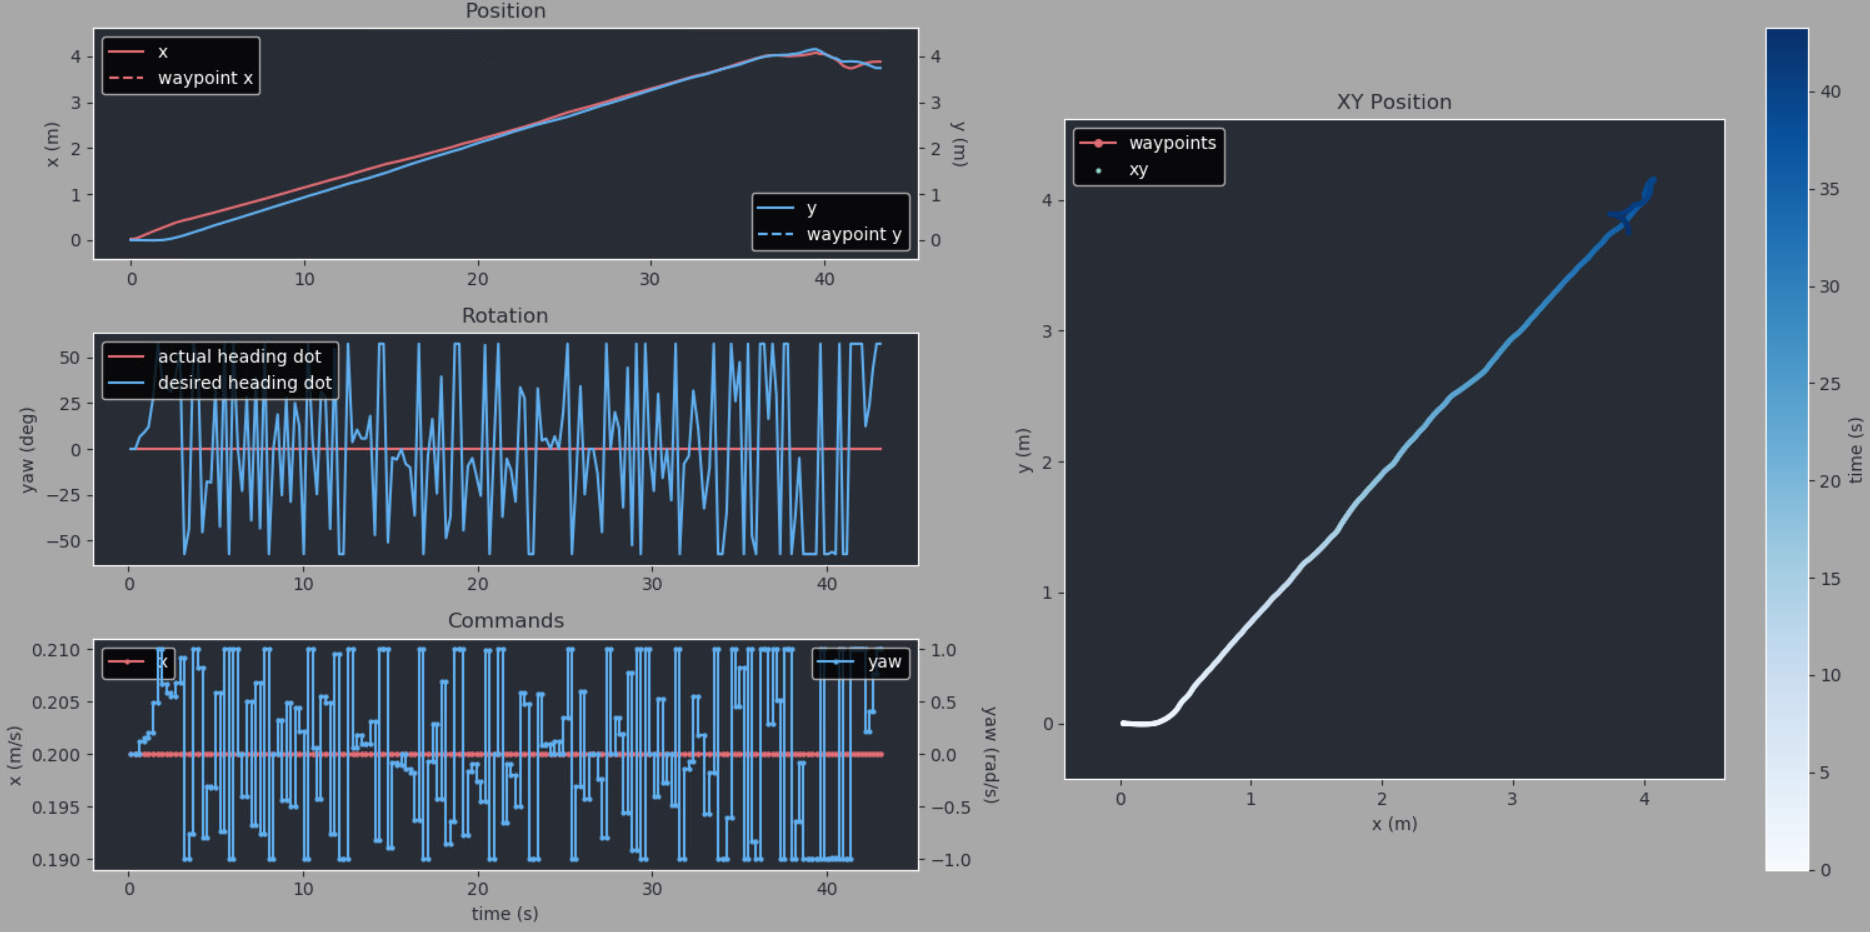
\includegraphics[width=\linewidth]{PN_0o15.png}
        
% % % % % % % % % % % % % % % % % % % % % % % % % % % % % % % % % % % % % % % % 
    \newpage
    \section*{Problem 2}
    Simply, if the gain is not high enough we won't hit the evader, but because we cap the max turn rate, we can get away with a high gain. \break
    Note: the max turn rate is set to 1.0, and not the actual limit of the turtle bot. \break

    \begin{center}
        PN = 0.015 \break
        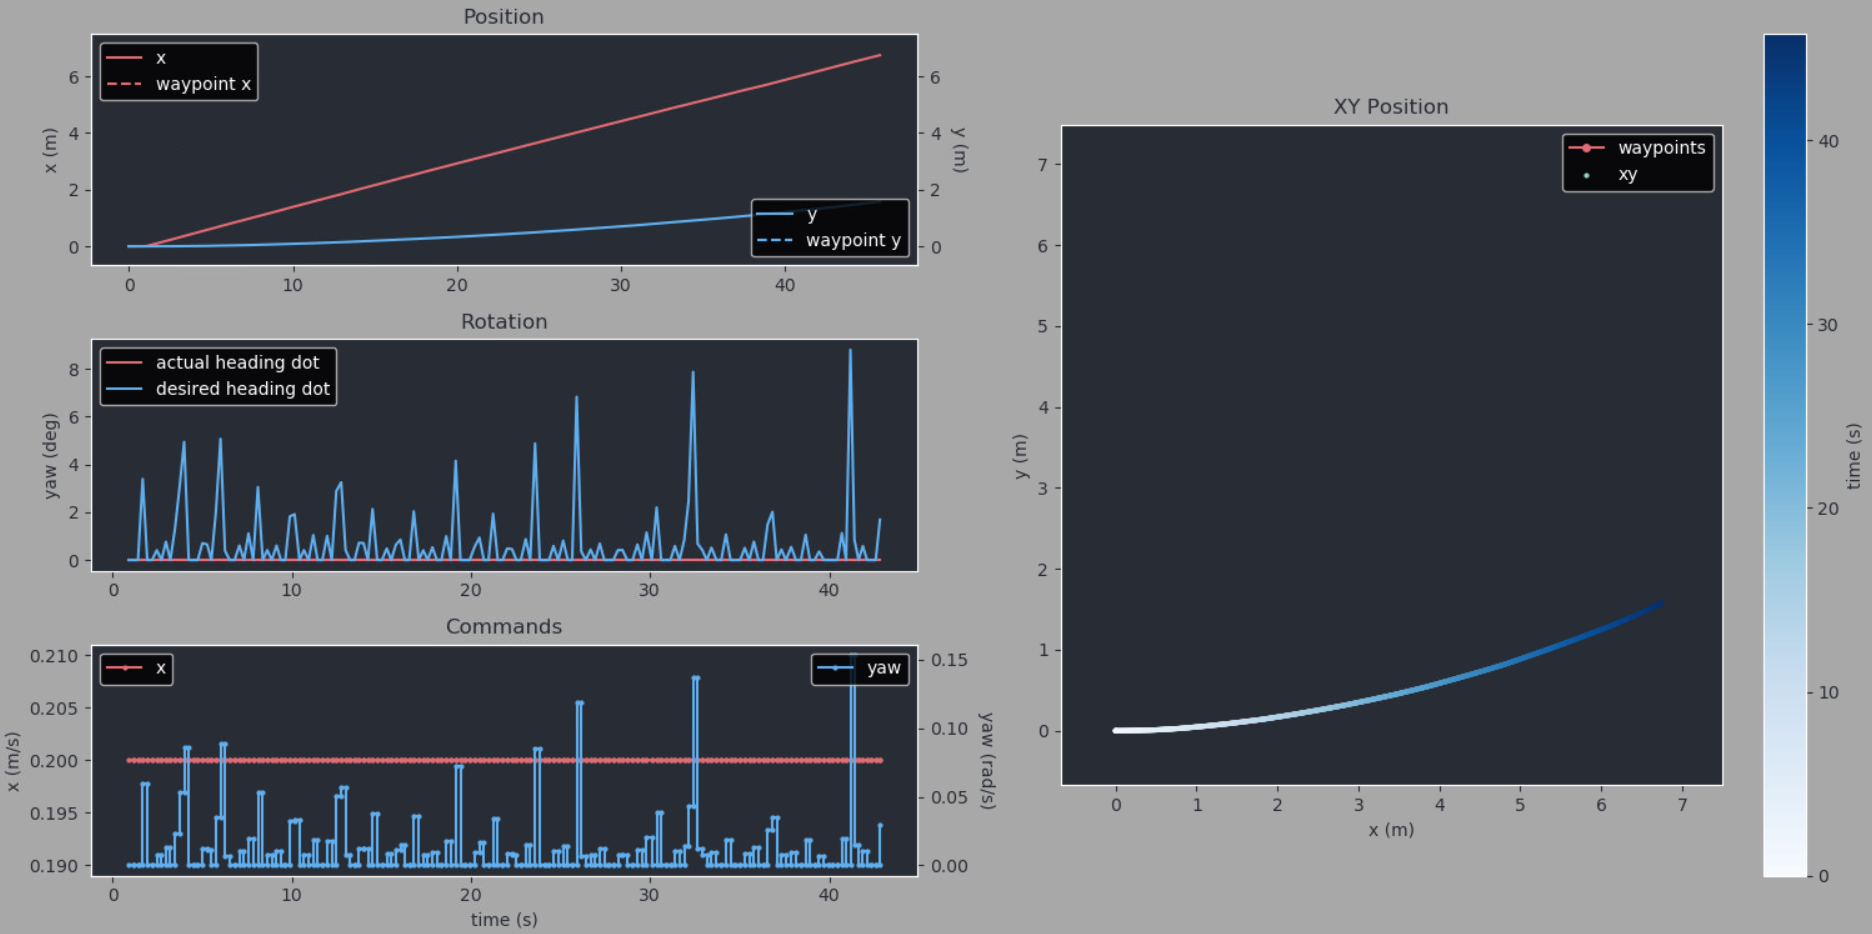
\includegraphics[width=4.7in]{PN_0o015.png}
    \end{center}

    \begin{center}
        PN = 0.15 \break
        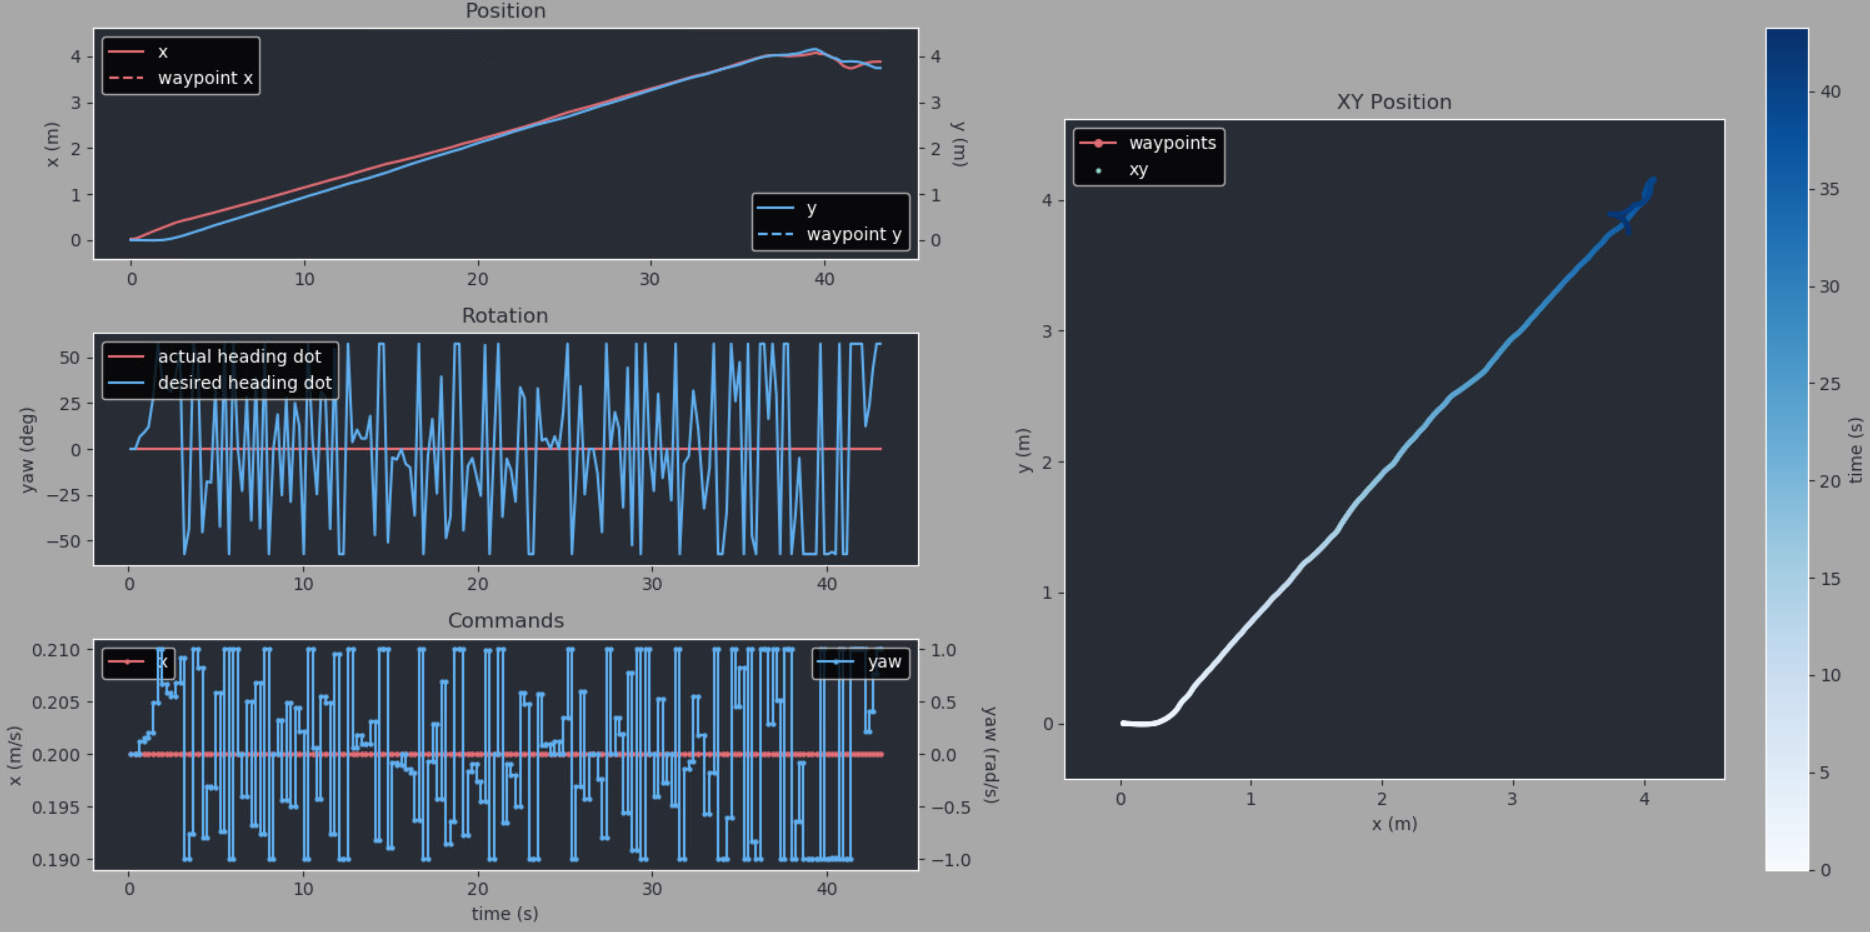
\includegraphics[width=4.7in]{PN_0o15.png}
    \end{center}

    \begin{center}
        PN = 1.5 \break
        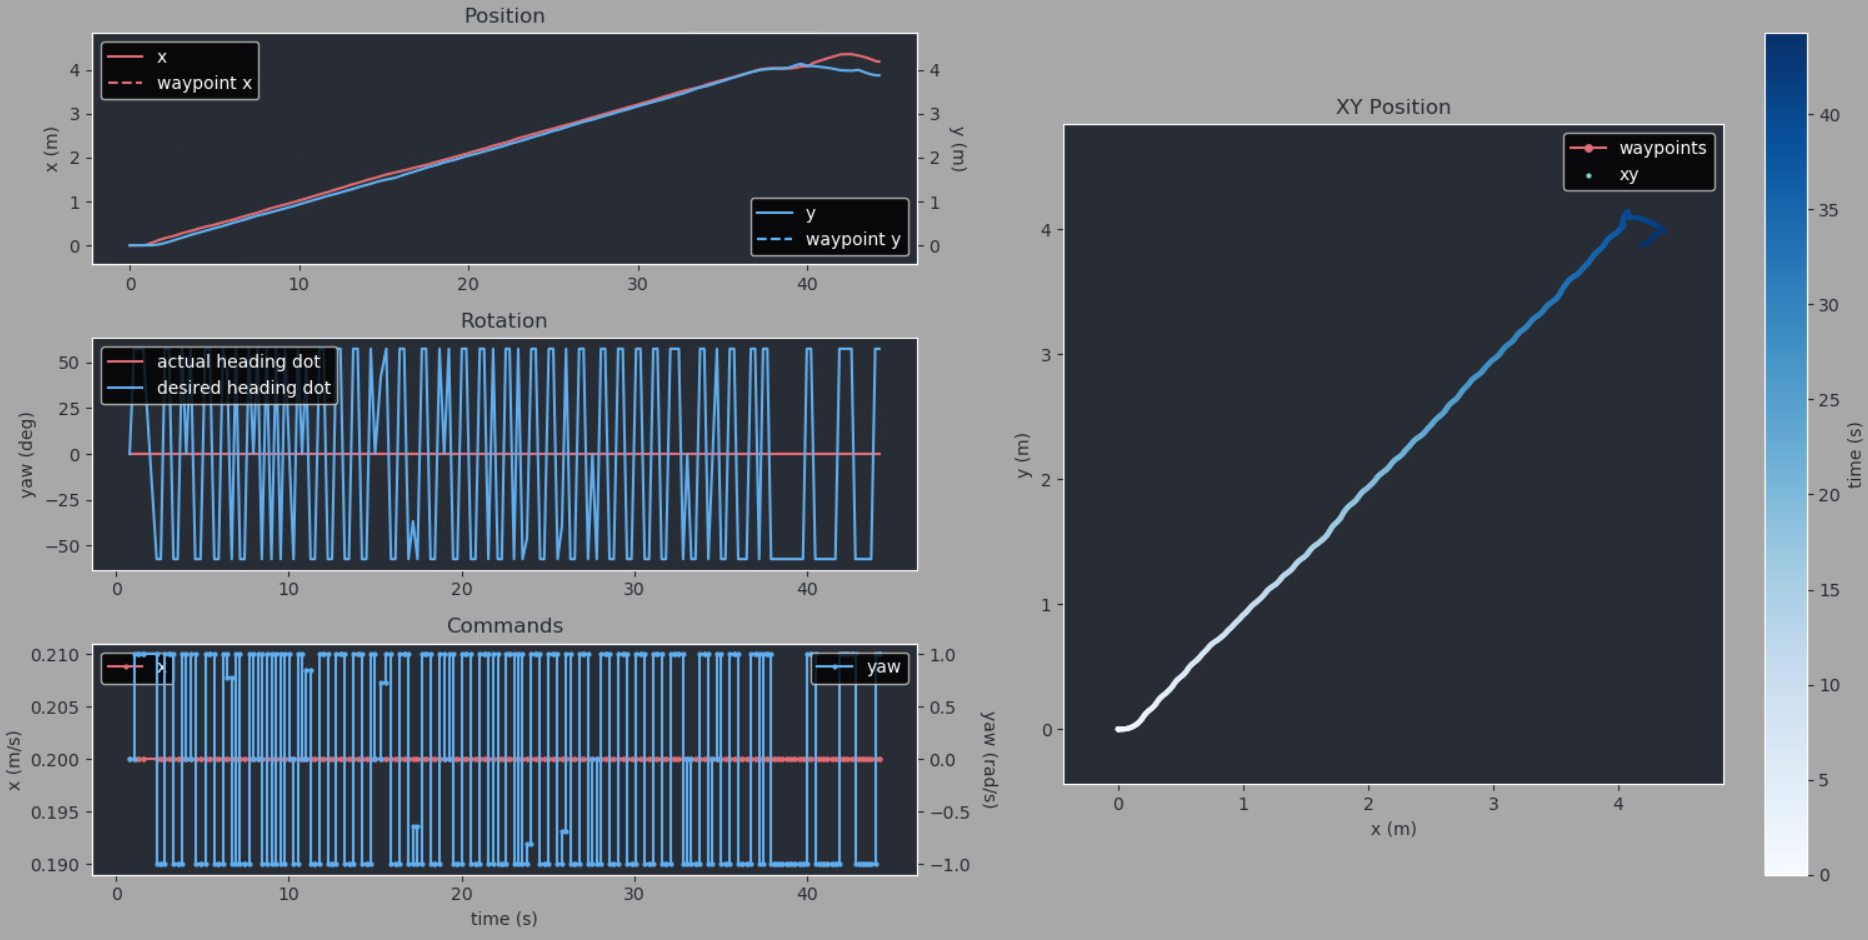
\includegraphics[width=4.7in]{PN_1o5.png}
    \end{center}
        
% % % % % % % % % % % % % % % % % % % % % % % % % % % % % % % % % % % % % % % % 
    \newpage
    \section*{Problem 3}

    My pursuer too good, evader doesn't get a chance to switch waypoints :smile: 

    \begin{center}
        pursuer \break
        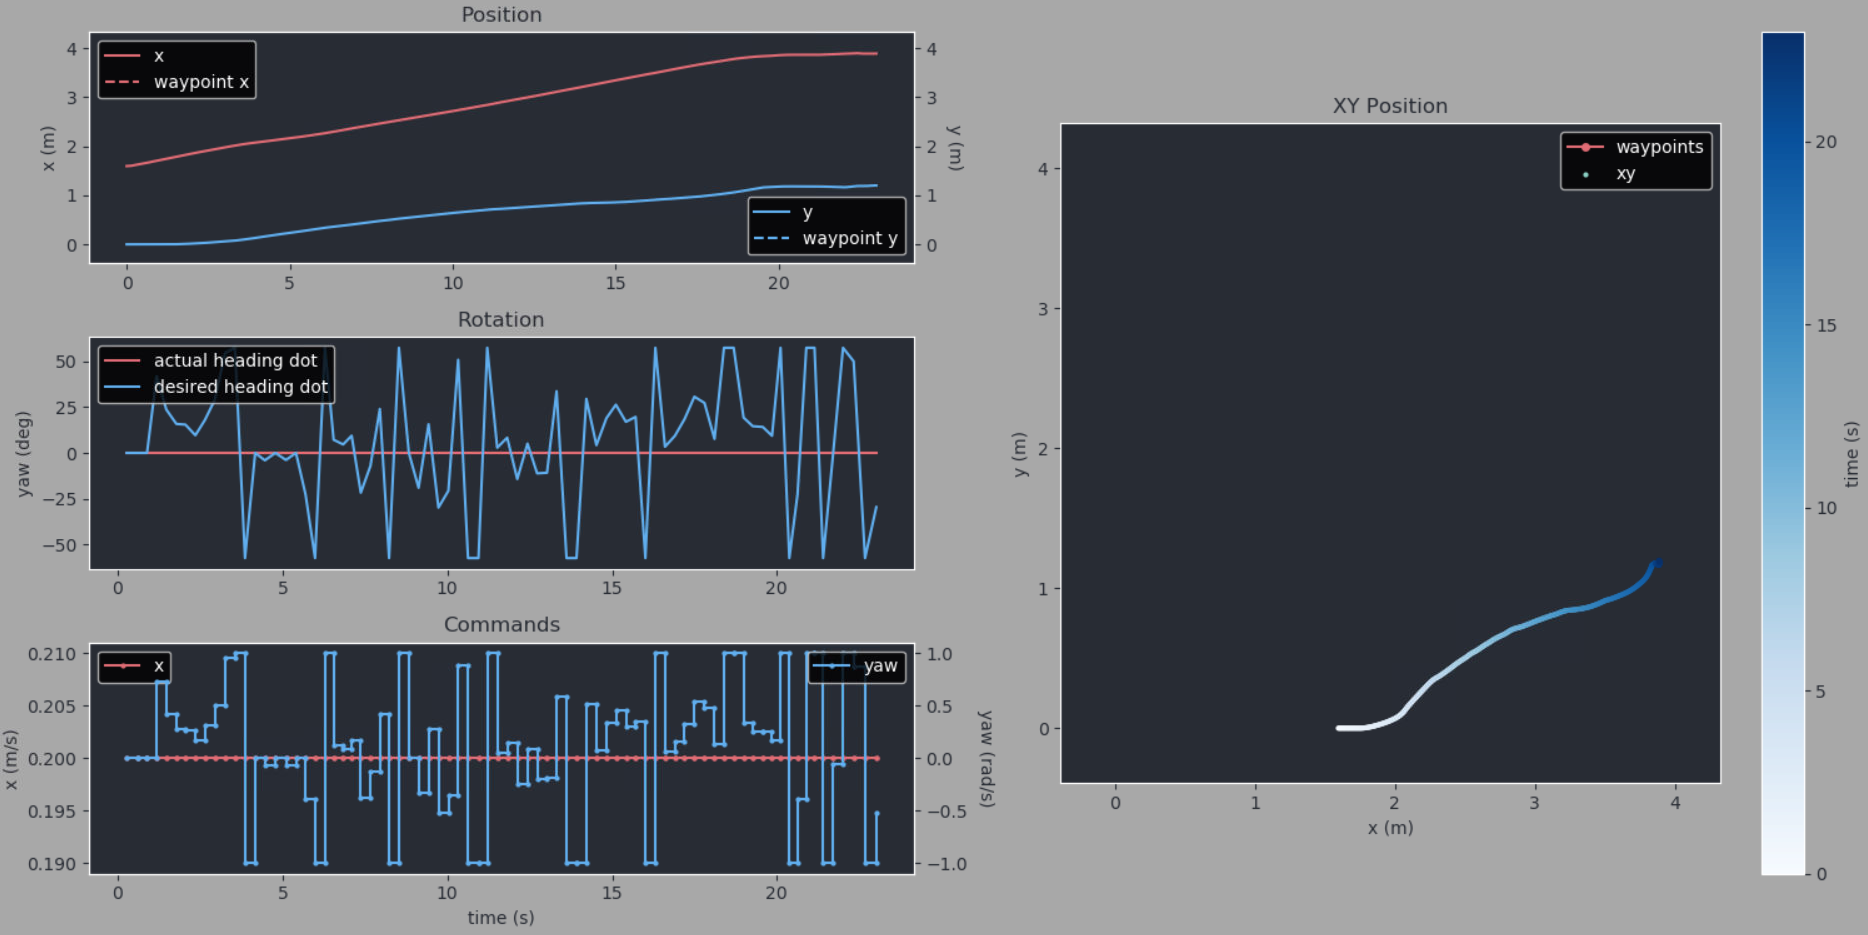
\includegraphics[width=5in]{pursuer_random_evader_1.png} \break

        evader \break
        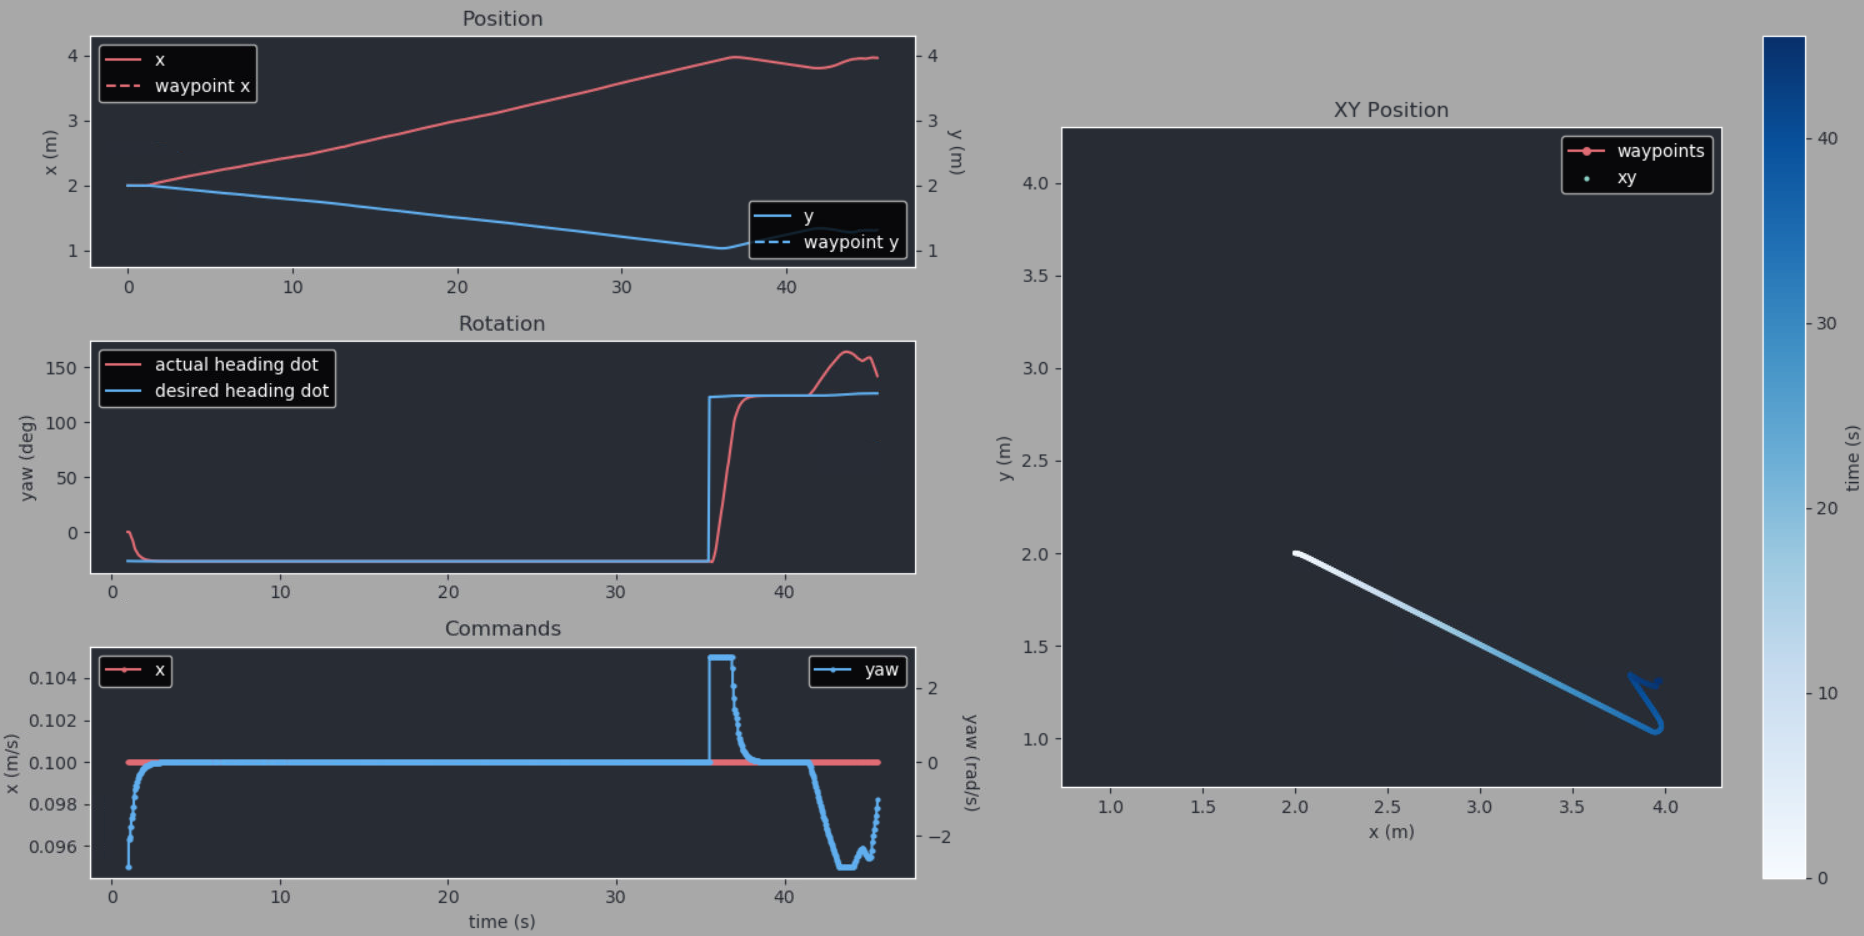
\includegraphics[width=5in]{evader_random_evader_1.png}
    \end{center}

    \newpage
    \begin{center}
        puruser \break
        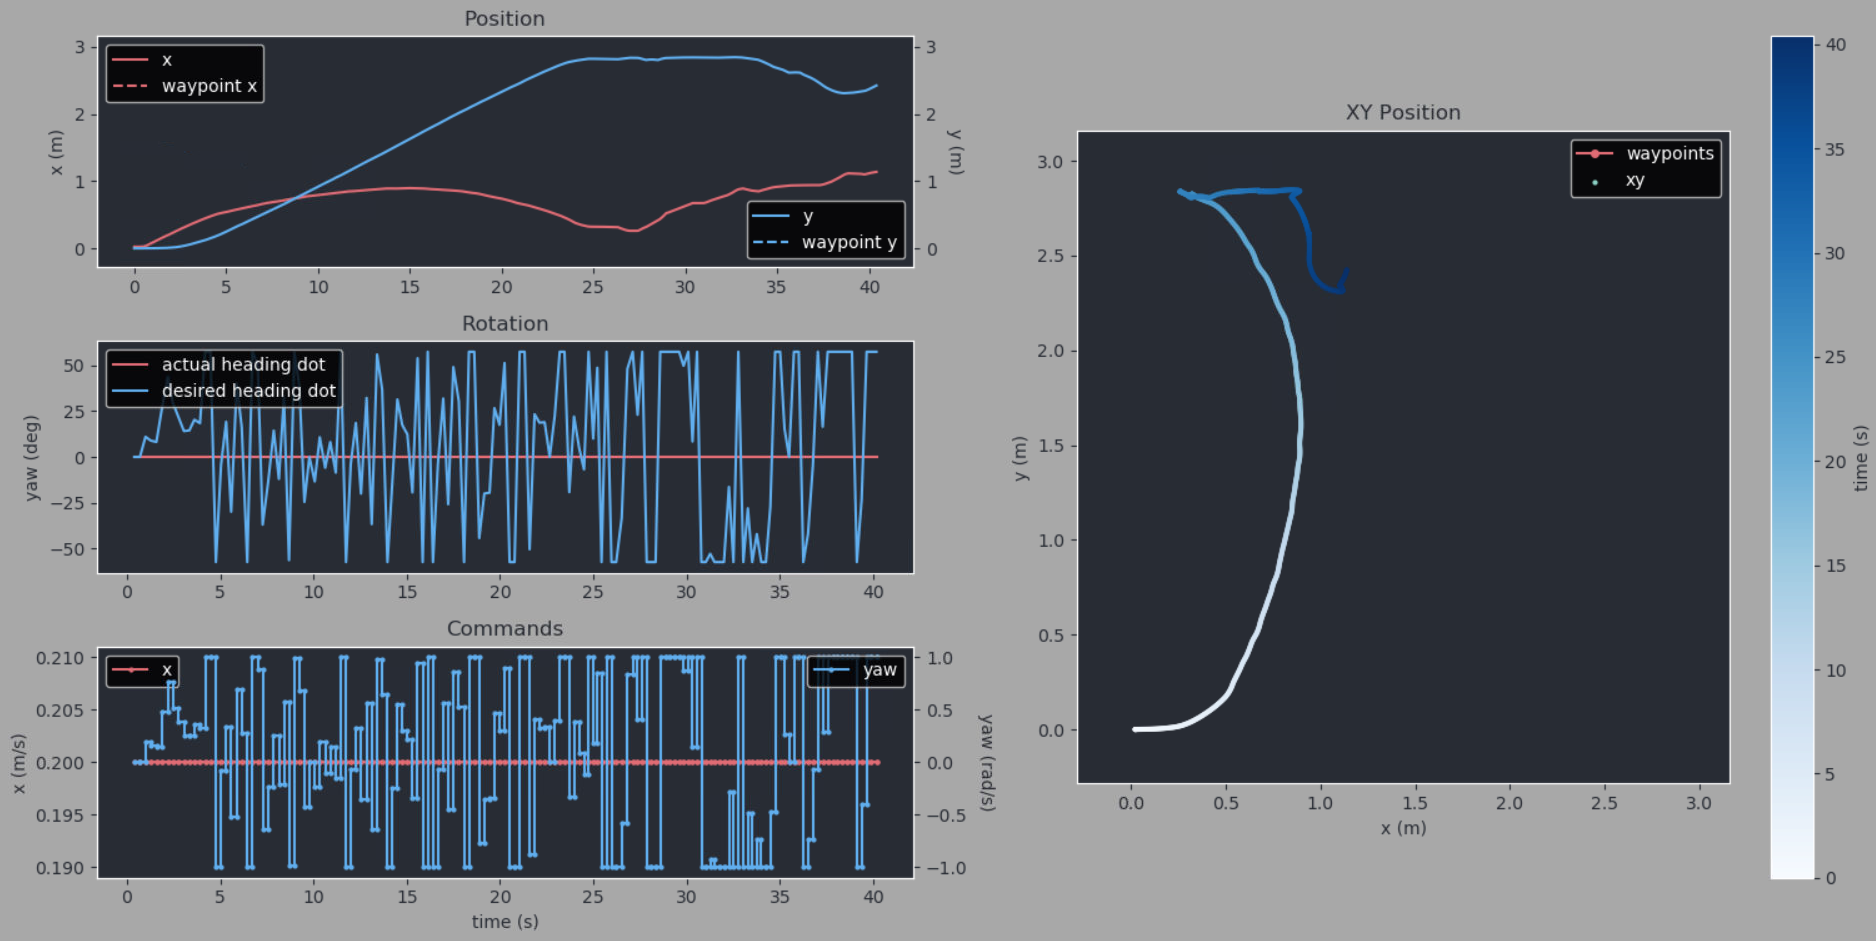
\includegraphics[width=5in]{pursuer_random_evader_2.png} \break

        evader \break
        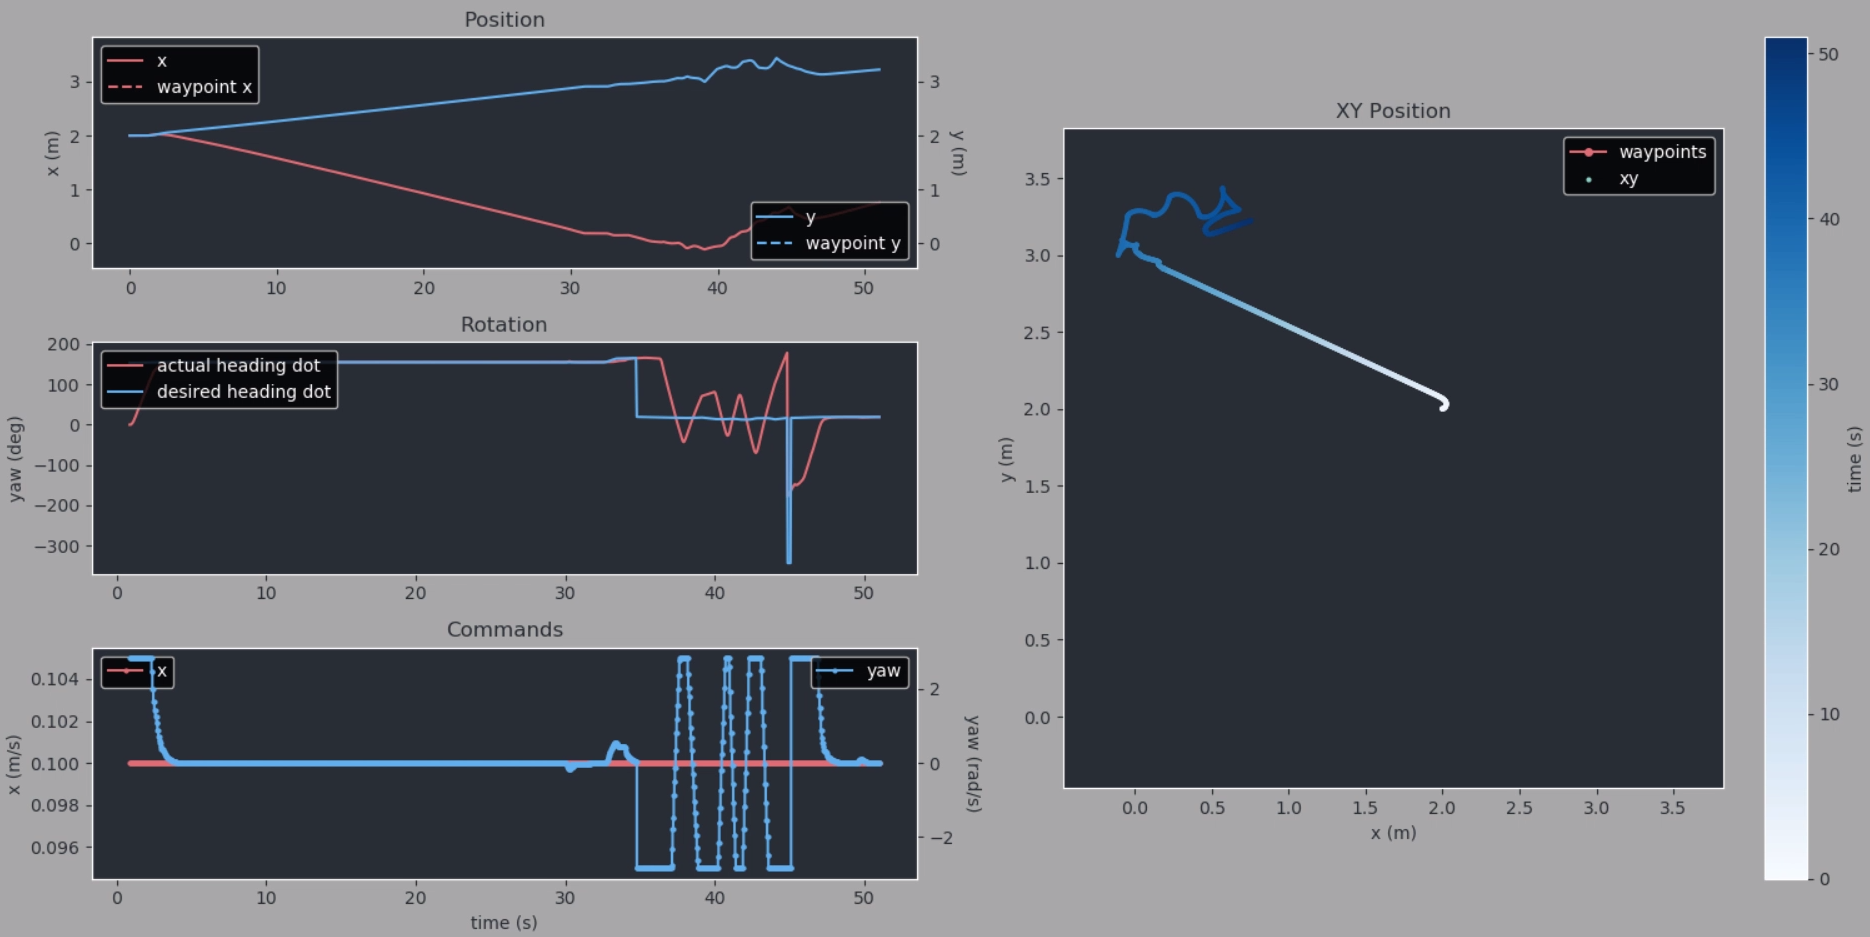
\includegraphics[width=5in]{evader_random_evader_2.png}
    \end{center}
        
% % % % % % % % % % % % % % % % % % % % % % % % % % % % % % % % % % % % % % % % 
    \newpage
    \section*{Problem 4}
    As long as the pursuer's PN gain or max turn rate is low enough, the evader can get away with half the speed. For this test, I kept the pursuer PN gain at 0.15, but nerfed the turn rate from 1.0 to 0.284 (one tenth of evader's max turn rate). However, to solve the max turn rate problem, puruser can just increase their PN gain to lead the target more, but there is a limit to this as eventually it'll just do circles trying to lead the evader indefinitely. \break

    Nonetheless, a good strategy for the evader is to keep the pursuer 90 degrees of its nose; this should ensure the tightest possible cirlce without intercepting the pursuer itself. \break
    So, the evasive logic is simply if the pursuer is within 1 meter, evade using the 90 degrees strategy, and hope the pursuer isn't as capable as you. \break

    Pursuer: \break
    Max turn rate: 0.284 \break
    PN Gain: 0.15 \break
    \begin{center}
        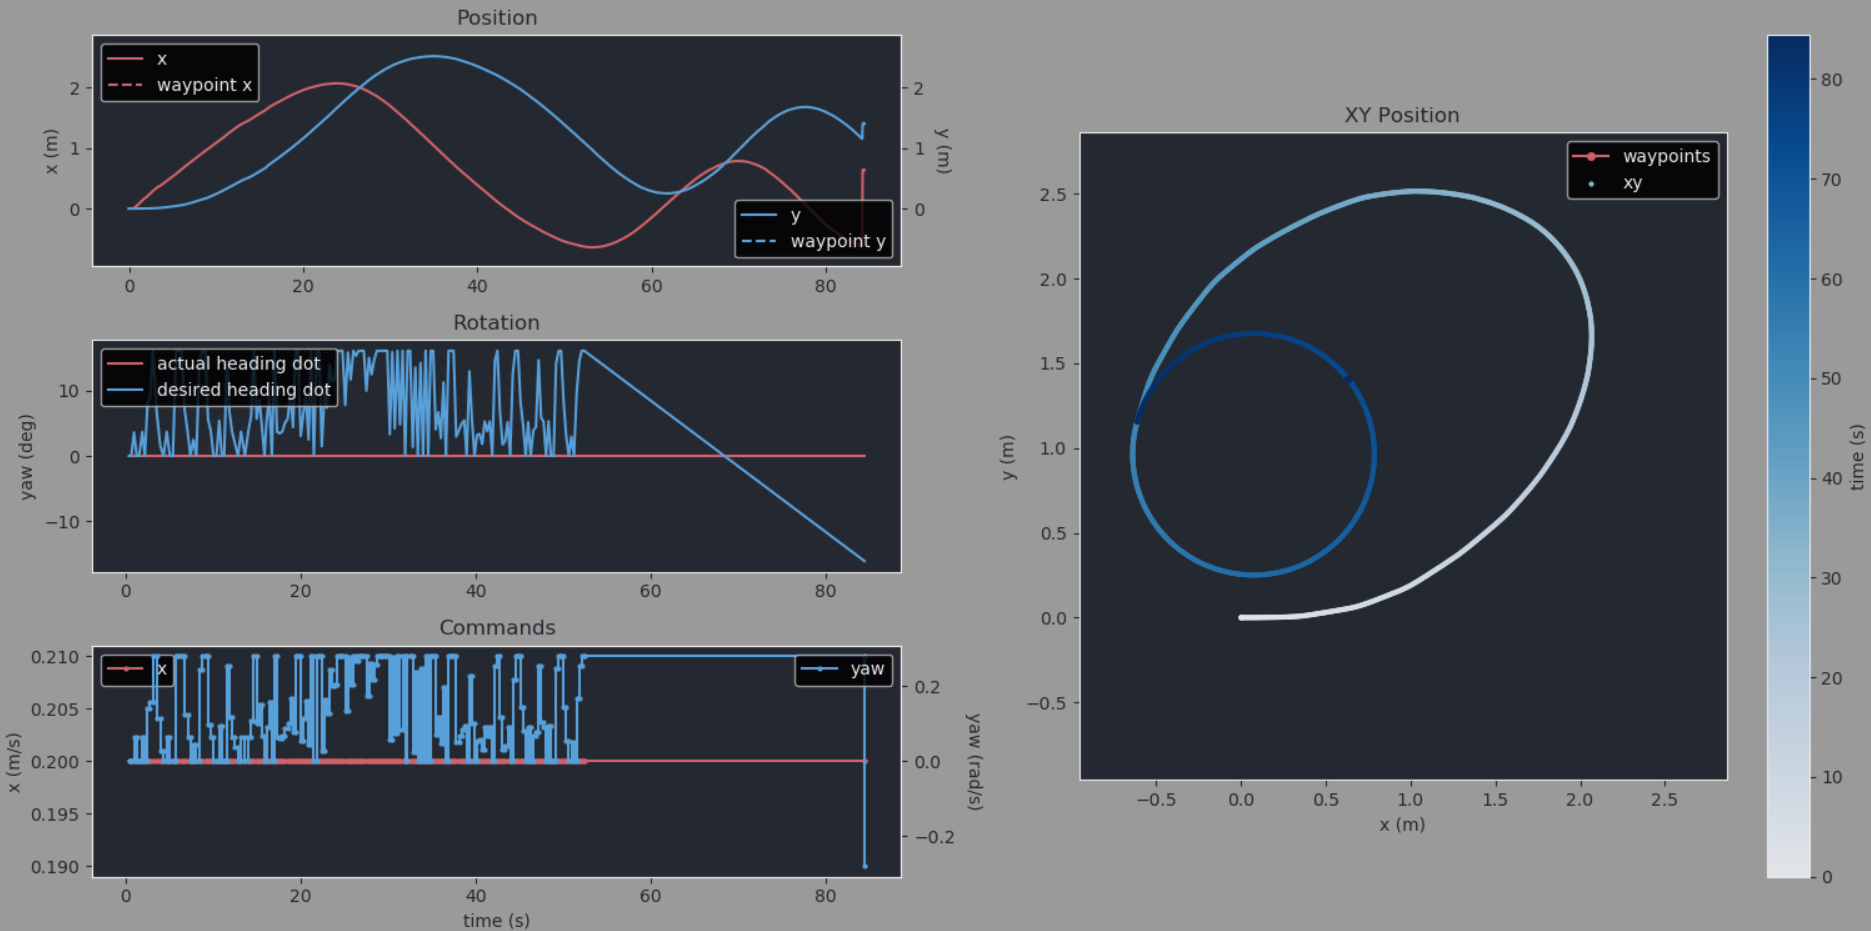
\includegraphics[width=5in]{puruser_bad_puruser.png}
    \end{center}

    Evader: \break
    Max turn rate: 2.84 \break
    \begin{center}
        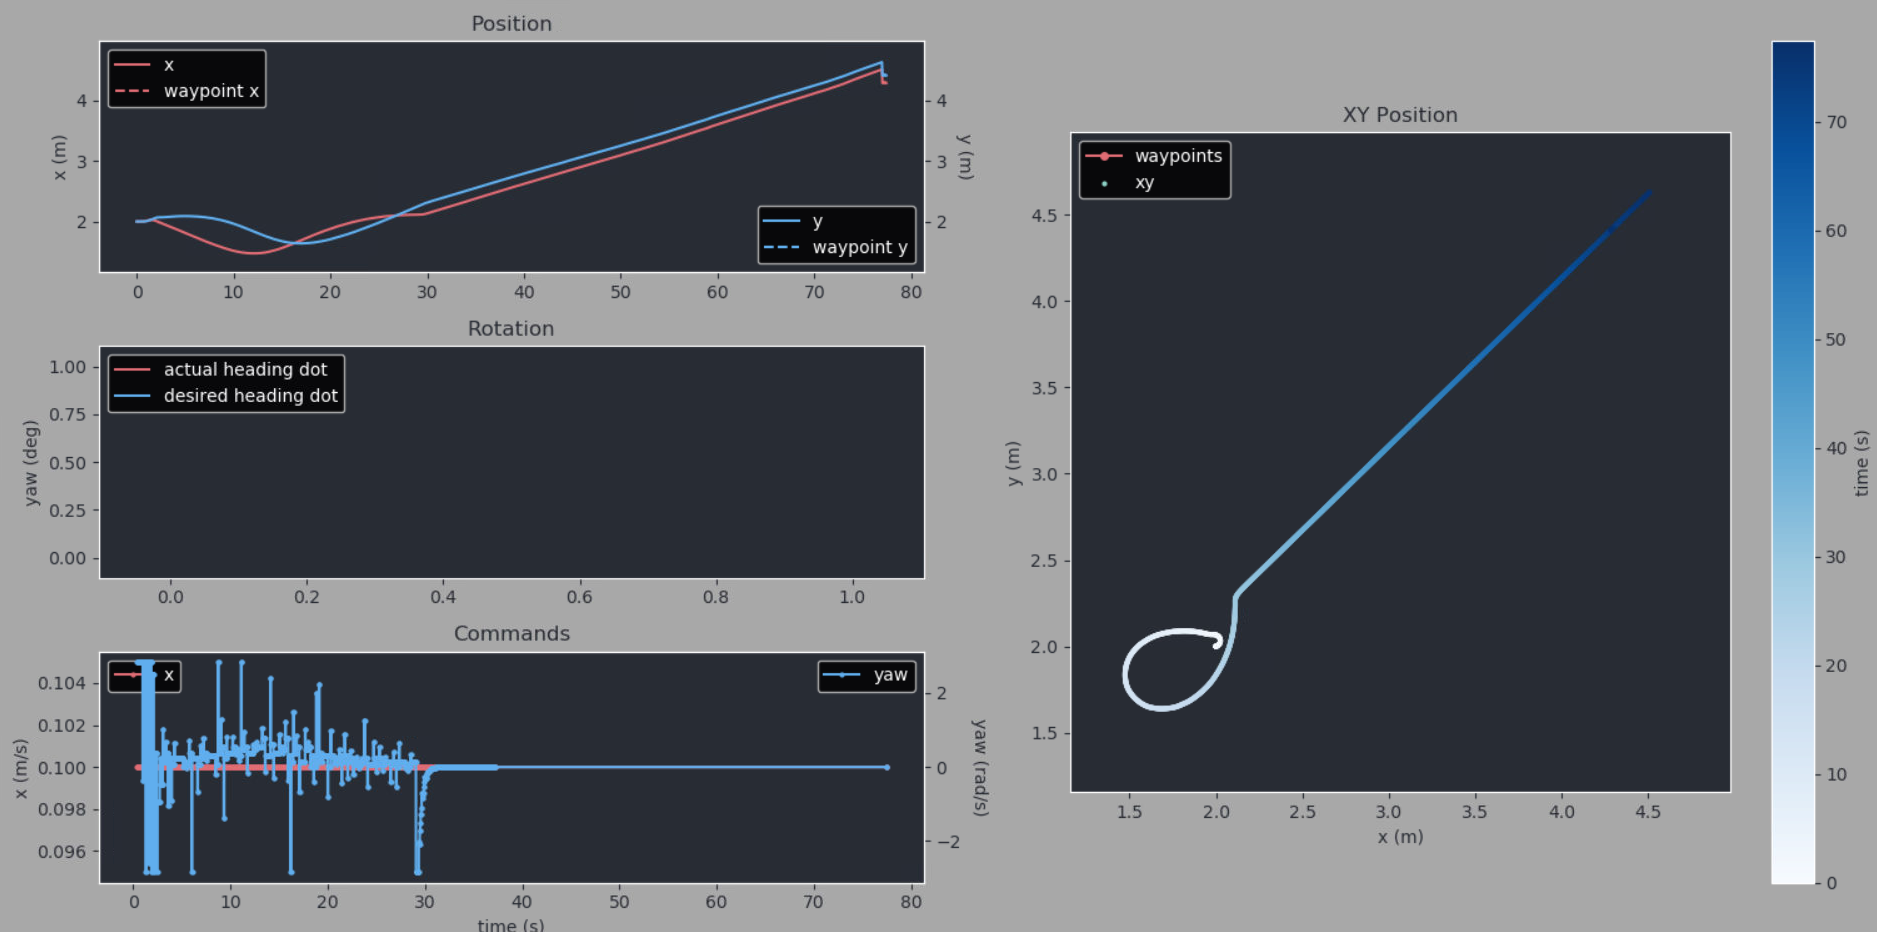
\includegraphics[width=5in]{evader_bad_pursuer.png}
    \end{center}
        
% % % % % % % % % % % % % % % % % % % % % % % % % % % % % % % % % % % % % % % % 
    \newpage
    \section*{Problem 5}
    Teddy cheated, he made his evader go zoom if puruser got close... :thumbsupdown: :D
    
% % % % % % % % % % % % % % % % % % % % % % % % % % % % % % % % % % % % % % % % 
    \section*{Problem 6}
    Problem 6 requires real turtlebots, something we never got to.

\end{document}